%%%%%%%%%%%%%%%%%%%%%%%%%%%%%%%%%%%%%%%%%%%%%%%%%%%%%%%%%%%%%%%%%%%%%%
% LaTeX Template: Project Titlepage
%
% Source: http://www.howtotex.com
% Date: April 2011
%
% This is a title page template which be used for articles & reports.
%
% Feel free to distribute this example, but please keep the referral
% to howtotex.com
%
%%%%%%%%%%%%%%%%%%%%%%%%%%%%%%%%%%%%%%%%%%%%%%%%%%%%%%%%%%%%%%%%%%%%%%
%
% --------------------------------------------------------------------
% Preamble
% --------------------------------------------------------------------

\documentclass[paper=a4, fontsize=11pt,twoside]{scrartcl}       % KOMA

\usepackage[a4paper,pdftex]{geometry}   % A4paper margins
\setlength{\oddsidemargin}{5mm}                 % Remove 'twosided' indentation
\setlength{\evensidemargin}{5mm}

\usepackage[english]{babel}
\usepackage[font=footnotesize, labelfont=it]{caption}
\usepackage[protrusion=true,expansion=true]{microtype}
\usepackage{mathtools}
\usepackage{graphicx}
\usepackage{wrapfig}
\usepackage{subfig}
\usepackage{amsfonts}
\usepackage[backref=true, sorting=none]{biblatex}
\usepackage{csquotes}
\addbibresource{bibliography.bib}
\usepackage{hyperref}
\hypersetup{
        colorlinks=true,
        linkcolor=blue,
        filecolor=magenta,
        urlcolor=blue,
        citecolor=blue
        }
\urlstyle{same}

% --------------------------------------------------------------------
% Definitions (do not change this)
% --------------------------------------------------------------------

\newcommand{\HRule}[1]{\rule{\linewidth}{#1}}   % Horizontal rule

\makeatletter                                                   % Title
\def\printtitle{%
    {\centering \@title\par}}
\makeatother

\makeatletter                                                   % Author
\def\printauthor{%
    {\centering \large \@author}}
\makeatother

% --------------------------------------------------------------------
% Metadata (Change this)
% --------------------------------------------------------------------

\title{
                        \HRule{0.5pt} \\                                                % Upper rule
                        \LARGE \textbf{\uppercase{A Computationally Tractable Model for the Evolution of a Genome's Size and its Growing Fitness Landscape}}      % Title
                        \HRule{2pt} \\ [0.5cm]          % Lower rule + 0.5cm spacing
                        \normalsize \today                      % Todays date
                }

\author{
                \textbf{Master's Thesis}\\
                Faculty of Science, University of Bern\\
                \vspace{1cm}
                Handed in by \\
                \textbf{Jacob Hugh Riina} \\
                \vfill
                Supervisors\\
                Prof. Dr. Claudia Bank\\
                Dr. Stephan Peischl\\
}

\begin{document}

% ------------------------------------------------------------------------------
% Maketitle
% ------------------------------------------------------------------------------

\thispagestyle{empty}           % Remove page numbering on this page

\printtitle                                     % Print the title data as defined above
        \vfill
\printauthor                            % Print the author data as defined above
\newpage

% ------------------------------------------------------------------------------
% Begin document
% ------------------------------------------------------------------------------

\setcounter{page}{1}            % Set page numbering to begin on this page

\section*{Introduction}

\subsection*{Genome Evolution}

Since life's origins approximately 3.5 billion years ago, it has generally increased in complexity, and understanding the processes that generate this complexity is one of the main goals of evolutionary biology. One such mechanism of generating complexity is through genome evolution: by changing the size of their genomes, the earliest living cells - those with a cell membrane, which encode and pass on information through their DNA - were able to create \textit{evolutionary innovations}: new metabolism, physiology or regulation, which augumented their ability to thrive in a variety of environments. At the increased cost of replicating and proofreading more DNA, organisms have since been able to evolve new genes allowing them to metabolize different carbon, nitrogen, or complex nutrient sources, various types of receptors and secretion systems to interact, competitively or mutualistically, with others, and the internal regulatory networks required for them to decide which behaviors are optimal under which circumstances, or even to coordinate multicellularity. Several billion years later, we see the consequences of this incessant evolutionary process: the stunning diversity amongst organisms in the tree of life, each a product of the series of environments they have adapted to. We can say, then, that the content of an organism's genome is not solely the result of how it has evolved to fit its current environment, but also the entire history of environments that its ancestors have evolved in; as always, "Nothing in biology makes sense except in the light of evolution".\\ 

Understanding this facet of evolution is difficult. Unlike with the point mutations that are typically observed in every generation, genome evolution occurs up to several orders of magnitude less frequently, and is more heterogenous in its manifestation. We define here genome evolution as a mutational process resulting in either the expansion or reduction in the size of the functional genome, arising from one of several causes: amongst genome-increasing mechanisms, there exist duplications from repeat region replication errors, transposon activity, or whole genome duplications (WGD), as well as genes arising from noncoding sequence through de novo gene birth, while genome-reducing mechanisms include pseudogenization and deletions via various types of replication errors. Evolution has been observed to utilize both genome reduction and expansion in order to spur adaptation to increase the organism's \textit{fitness}, conceptualized as some metric representing success e.g. growth rate within an environment. However, more impactful processes such as neofunctionalization of duplications, de novo gene birth, and WGD, remain slow to induce and test, often in experiments running for years or decades. There is thus a usefulness to the creation of mathematical models that bridge the gap between theory and experiment and allow us to form hypotheses about these phenomena and their impact over long evolutionary timescales.\\

One such [question] naturally arising from the study of this type of adaptive system is regarding the effects of \textit{path dependency} during genome evolution: how does the order and timing in which evolutionary innovations arise affect evolutionary possibilities far in the future, potentially in different environments? For instance, the nitrogenase metalloenzyme - the main driver of bioavailable nitrogen cycling, which utilizes multiple oxygen-labile iron-sulfur clusters - emerged under the earth's early atmospheric conditions and favored adaptations suited to a reducing atmosphere. Faced with a later change to an oxidizing and highly destructive environment, organisms with this metabolic innovation, incapable of decommitting from fixing their own nitrogen to sustain cell growth, instead evolved a set of highly complicated cellular pathways to continue catalysis under only anoxic conditions, and protect the enzyme's metallic core from molecular oxygen. No other method of creating bioavailable nitrogen in an oxygenic cellular environment has ever been discovered. What if nitrogen fixation had first evolved after the oxygenation of the atmosphere? Is it even possible, and if so, how would the enzyme differ from today's? Evolution appears to be rife with examples of historical contingencies, spanning from within microbial metabolism up to macroscale physiology[cite giraffe]. [these are questions about the evolution of genomic context over time, and therefore a good starting point is from mathematical models that allow for the modeling of context, and how it can evolve. We thus turn to fitness landscapes.] how do different cellular contexts create different evolutionary outcomes, which then lead to even more different contexts, which lead to even different outcomes?

\subsection*{Fitness Landscape Theory}

The fitness landscape was first introduced in 19xx by Sewall Wright to illustrate xyz. With each unique combination of decisions there can be assigned a fitness value, and so we can generate a topology from a network of possible decision combinations. Fitnesses for contexts on the landscape may be higher or lower than expected from the sum of their individual components, leading to "ruggedness", otherwise known as \textit{epistasis}: nonadditivity resulting from higher-order interactions between components, that ultimately leads to, in the case of evolution, adapting populations reaching differing and suboptimal equilibrium points as they perform a "hill-climbing" style of optimization. This analogy has spurred a great deal of research in evolutionary biology, where it has found use in modeling adaptation of alleles, or more recently, in empirical fitness landscapes of proteins. The model can in fact be generalized to represent any sort of decision landscape, and has consequently found itself applied broadly in variety of fields such as [Directed evolution, economics?, and the other one]. Although fitness landscape theory has been used extensively to model adaptation on static genomes or within changing environments, it is less well developed on the scale of long term evolution, where changes in genomic context also arise and can be selected for. With this work we extend the Rough Mount Fuji model to incorporate genome evolution alongside allelic mutation to explore the effects of multiple mutational processes on evolutionary outcomes.

\section*{Methods}

\subsection*{The Rough Mount Fuji Model}

The Rough Mount Fuji (RMF) model allows for tunable epistasis \cite{neidhartAdaptationTunablyRugged2014} and so enables the investigation its effects as landscapes scale. In this model we represent genotypes as binary vectors, and their permutations in genotype space construct a network where each has a hamming distance of 1 from its neighbors, and the degree of each node is equivalent to the number of loci $L$ in the model (see Figure~\ref{fig:genotype_space}).

The assignment of fitness values to genotypes entails sampling two probabilistically determined components: Locus-wise additive effects $a = (a_1, \cdots, a_i) \sim \text{iid. } \mathcal{N}(0, 1)$ are drawn from a normal distribution, and each genotype $g$ recieves a unique epistatic component $e_g \sim \mathcal{N}(0, \sigma_e)$, also drawn from a normal distribution.  Fitness values for some arbitrary genotype can then be assigned as the sum of the product of the additive effects and the genotype, plus the epistatic component, as an exponential: $$f_g = exp{(e_g + \sum_{i=0}^{L} a_i * g_i)}$$ Epistasis is represented in the ratio between the variance of additive components and epistatic components, and we control epistasis on the landscape by varying the epistatic $\sigma_e$ - in cases where the epistatic component is small the additive component dominates and the landscape becomes easily predictable, whereas when epistatic effects are large and outweigh the additive component, there is virtually no correlation between different genotypes and ruggedness is high. Now able to reproducibly retrieve some epistatic component for any genotype by providing the CBRNG with the base-10 representation of that binary genotype, we are no longer obligated to generate fitnesses for all genotypes on the landscape in advance and instead need only do so upon encountering that genotype during simulation.

A discrete-generation RMF model with Wright-Fisher dynamics was implemented based on \cite{liRapidAdaptationRecombining2024} and previous software \cite{amadoSTUNForwardtimeSimulation2023}. We model a static $N$ total individuals mutating and reproducing simultaneously in each generation, with genotype frequencies governed by binomial and multinomial sampling, respectively. To initialize the simulation, we specify the number of loci in the model and consequently the length of the vector of additive effects to generate, the number of randomly distributed initial genotypes on the landscape and the number of individuals per genotype, the simulation length, the variance $\sigma$ of the epistatic component, and the mutation rate $\mu$ - the probability for an individual to generate a mutant of hamming distance 1 from its parent. An initial report table is then generated with a description of initial genotypes on the landscape, their population sizes, and fitnesses. We proceed to instantiate subsequent generations by first generating mutants from each extant genotype with population $\mathbb{P}$ through binomial sampling: $\text{Binomial}(n = \mathbb{P}, p = \mu)$. We adjust the corresponding population counts and calculate fitnesses for new genotypes if necessary, and then assign from $i$ extant genotypes for all individuals in the new generation of size $N$ new genotypes according to relative fitness: $\text{Multinomial}(N, p^{\prime} = (p^{\prime}_1, \cdots, p^{\prime}_i))$ given $p^{\prime}_i = p_i * \frac{\omega_i}{\bar{\omega}}$, where $p_i$ is some genotype's current frequency, $\omega_i$ is its fitness, and $\bar{\omega}$ is the average fitness across all extant genotypes. Therefore, highly fit mutants gain an advantage during sampling and are less likely to be eliminated through drift. The simulation is run for the specified number of generations and upon terminating a final report is also provided (Figure~\ref{fig:report}).

\subsection*{Counter-Based Random Number Generation}

The facile generation of random epistatic components was performed using a Julia implementation \cite{JuliaRandomRandom123jl2024} of the Random123 package from D.E. Shaw Research \cite{salmonParallelRandomNumbers2011}. Particularly, the ARS1x generator was used, with a period of $2^{128}$, this being the number of loci that can be modeled in a genotype network without reseeding.

\subsection*{Scripting}

\section*{Results}

\subsection*{Additive Limit}

We examine first the simple case where $\sigma_{e}$ is zero, resulting in a monopeaked landscape with no epistasis. Simulations were initialized with the following parameters, and xxx replicates were run by varying the seed value for the mutational rng.
\begin{center}
    \begin{tabular}{ | c | c | }
	\hline
	Maximum Size & 20 \\ \hline
	Initial Size & 1, 10, 20 \\ \hline
	Population & 1000 \\ \hline
	Generations & 50000 \\ \hline
	$\sigma_e$ & 0 \\ \hline
	$\sigma_a$ & 0.1 \\ \hline
	$\mu$  & 1e-4 \\ \hline
	$M$ & 1e-4 \\ \hline
    \end{tabular}
\end{center}

As there is no epistasis, populations will rapidly reach equilibrium at the fitness maximum on any individual landscape, whereas to find the global peak between all lanscapes a slighly different behavior is observed. Since a mutation to $0$ in either the genotype or genome produces an identical fitness, on average $50\%$ of negative additive effects will be removed via each type of mutation, and this balance will gradually fluctuate. Figure \ref{additivedynamics} shows genome sizes over time for starting genome sizes 1, 10, and 20 on a landscape with 10 positive additive effects. 

\begin{figure}
	\centering
	\subfloat[1 locus initially accessible]{\includegraphics[width = 0.4\textwidth]{figures/L20l1i1_20250901_1230_cropped.pdf}}
	\label{fig:sub1}
	\subfloat[10 loci initially accessible]{\includegraphics[width = 0.4\textwidth]{figures/L20l10i1_20250901_1229_cropped.pdf}}
	\label{fig:sub2}
	\subfloat[20 loci initially accessible]{\includegraphics[width = 0.4\textwidth]{figures/L20l20i1_20250901_1229_cropped.pdf}}
	\label{fig:sub3}
	\subfloat[Densities of genome size time series]{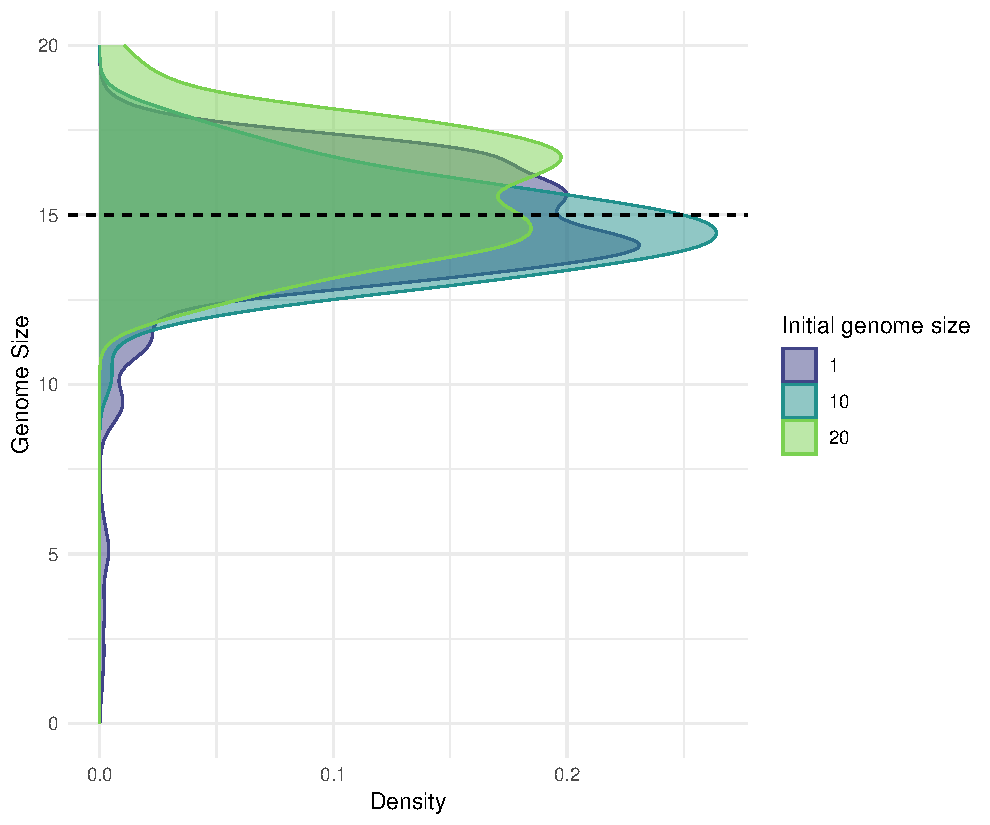
\includegraphics[width = 0.4\textwidth]{figures/random_walk_additive.pdf}}
	\label{additivedynamics:sub4}
	\caption{caption}
	\label{additivedynamics}
\end{figure}

It can be seen that fitness reaches the same value in all three cases within relatively few generations, while genome size simultaneously moves to and thereafter fluctuates about 75\% of the maximum. This can be attributed to the random swapping of the two fitness-equivalent mutations as described above, while maintaining a $1$ state for all positive effects. In this example, the 10 positive additive effects will always be on, and on average, out of the remaining ten negative additive effects, five will be not present in the genome, while five will be and mutated to a $0$ state, resulting in a mean genome size of 15 averaged over the entire time series (Figure \ref{additivedynamics}d). 

\subsection*{Uncorrelated Limit}

\subsection*{Time-Dynamic Outputs}

\subsection*{Endpoint Outputs}

Does endpoint exist under this model?

\section*{Discussion}

As has been noted by studies of the \textit{de novo} evolution of genes, their emergence out of unused genetic substrate remains difficult to observe experimentally. (why? duplication vs de novo navigation of landscapes).

Owing to a large protein fold space, evolution has generally favored mechanisms of duplication and neofunctionalization amongst new genes through horizontal gene transfer, transposon activity, or whole-genome duplications. (by doing so the cell acheives two things: 1. relieve pleiotropic effects, 2. lessen time to navigate sequence space). Alternatively, unused regions of the geome may also see genes spontaneously arise. (this process is much slower and harder to observe). In either case, these new genes are expected to accumulate neutrally, and over time have the opportunity to gain beneficial functionality.
Although organisms are effective at removing unnecessary genes through pseudogenization, (this is a slow process, and still does not account for historical contingencies)
Different organisms may happen to adapt to the same environment in different way

Implications on the expanding genome

\section*{Code and Data Availability}

\printbibliography

\end{document}



